%!TEX program=luatex

\newpage
\section{Introduction}
La réalisation d'un logiciel ou d'un système informatique doit être obligatoirement précédée d'une étape d'analyse et de conception qui a pour objectif de définir et de formaliser les étapes nécessaires du développement de l'application afin de rendre cette dernière plus fidèle aux besoins.

La première motivation de ce travail été de fournir un outil qui enchaîne les processus de catégorisation de résumé, de traduction et de recommandation d'articles de presse. Pour parvenir à réaliser cet ensemble de tâches en deux langues (Anglais et Arabe), nous proposons une architecture 3-tiers. 
\section{Architecture de "Feedny"}
L'architecture globale du système "Feedny" comporte quatre processus principales: Catégorisation, résumé, traduction et recommandation d'articles de presse.

Les entrées (articles de presse extraits de plusieurs sources) sont sauvegardés dans une base de données. Le processus de catégorisation commence par classifier l'article selon son contenu, ensuite un résumé est généré, l'article est traduit de l'Anglais vers l'Arabe (ou l'inverse) et enfin, il sera recommandé à un utilisateur selon son profile et ses préférences comme on peut le voir dans la figure \ref{shemaglobal}.

\begin{figure}[H]
    \centering
    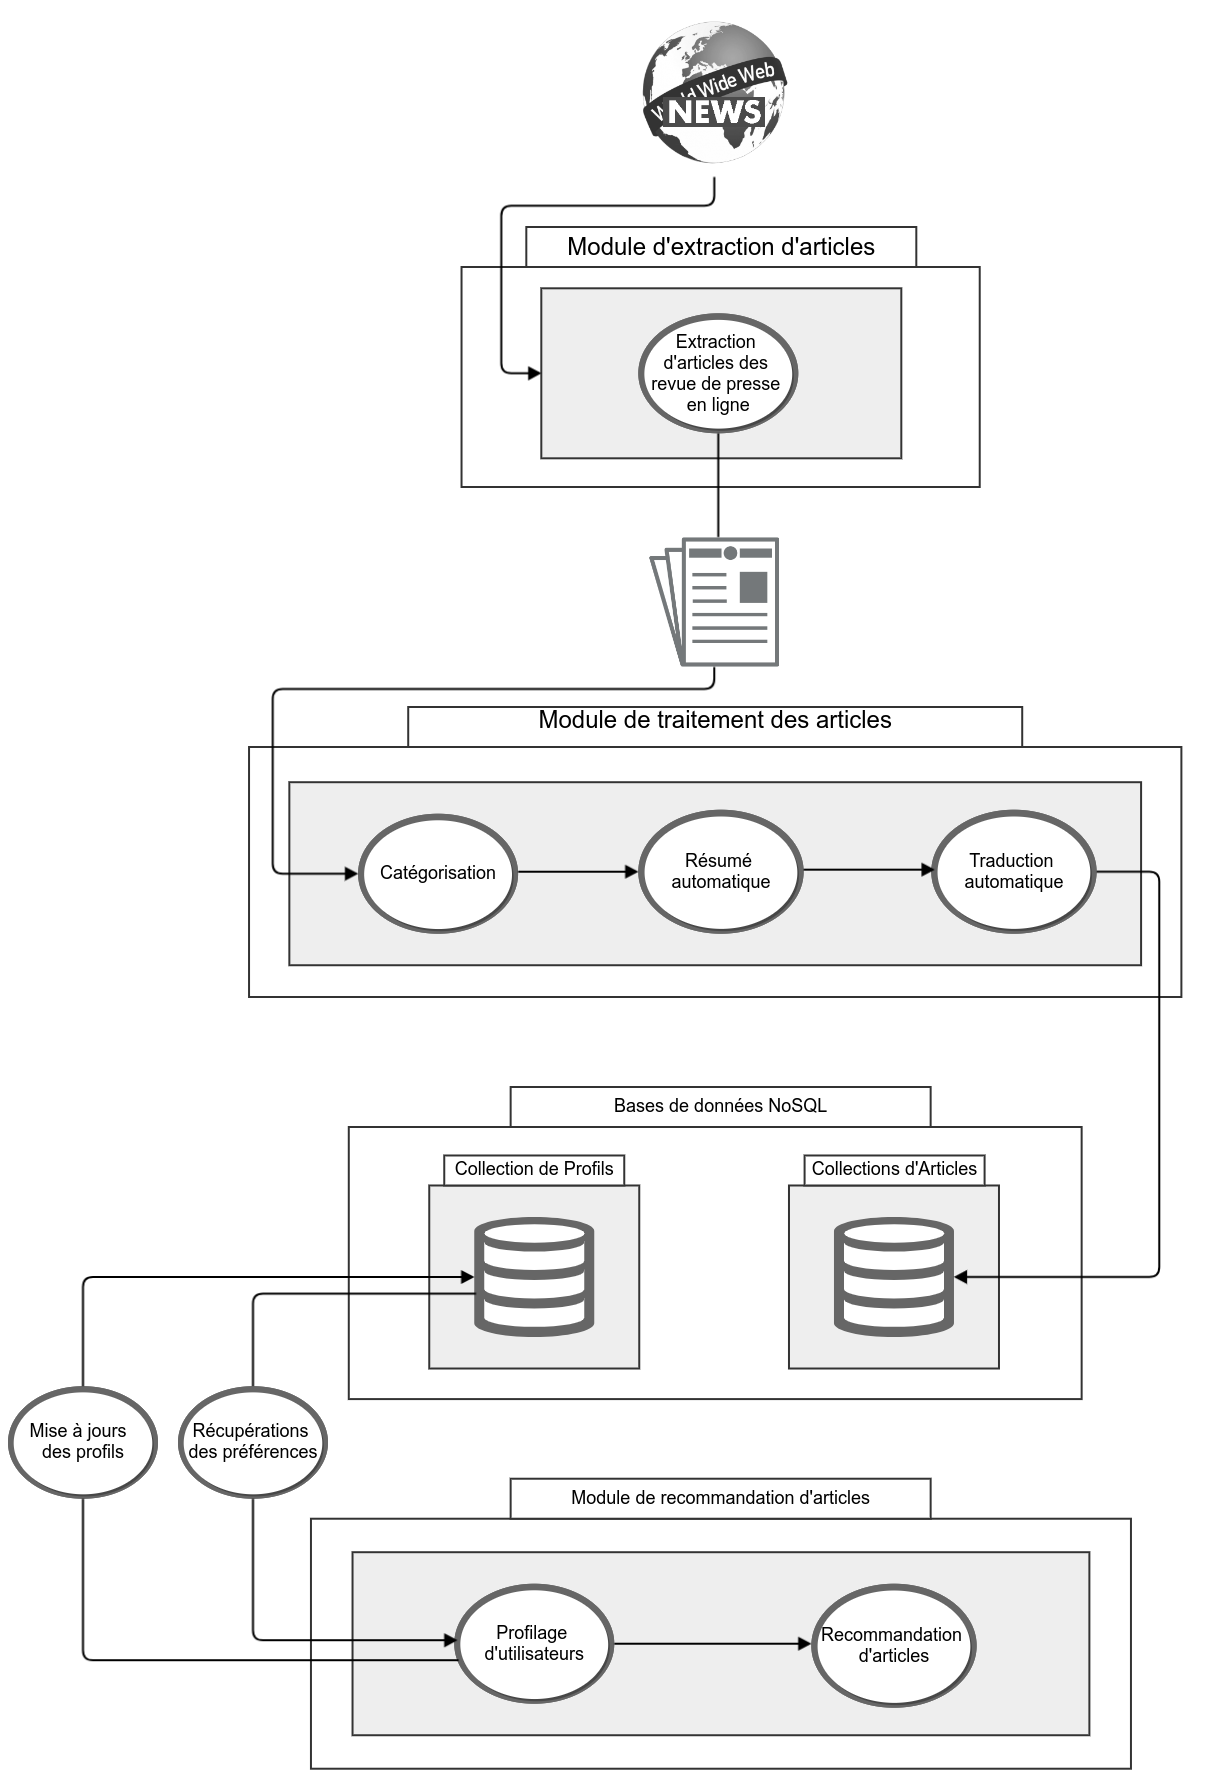
\includegraphics[height=320pt,width=330pt]{img/chapter3/global.png}
    \caption{Architecture globale du système.}
    \label{shemaglobal}
\end{figure}

\subsection{Stockage d'articles}
Les articles extraits depuis différentes sources sont tous sauvegardés sous une structure définie au préalable, prenant en considération les différences entre les formats suivies par les revu de presse. 

À cet effet nous avons choisi \emph{JSON} qui est un format léger d'échange de données. Il est facile à lire ou à écrire pour des humains\cite{json} et est pris en charge par tout les langages de programmation. 
Chaque article est représenté comme suit:
   \begin{itemize}
     \item \textbf{Identifiant "\_id": } identifiant unique.
     \item \textbf{Langue "language":} la langue dans laquelle l'article est écrit.
     \item \textbf{Titre "title":} le titre de l'article.
     \item \textbf{Source "source":} nom de la revue de presse source.
     \item \textbf{Auteur "author":} on sauvegarde le nom de l'auteur.
     \item \textbf{Contenu "content":} contenu de l'article.
     \item \textbf{Horaire "publishedAt":} Date et heur local de publication.
     \item \textbf{Lien de l'article "url":} lien vers la page de l'article originale.
     \item \textbf{Lien de l'image "urlToImage":} lien vers l'image principale de l'article originale.
     \item \textbf{Catégorie "categoryPredicted":} catégorie de l'article inférée en utilisant nos modèles.
     \item \textbf{Résumé "summaryGenerated":} résumé automatique générée.
     \item \textbf{Traduction "translatedContent":} contenu traduit.
    \end{itemize}
   
\subsection{Stockage de profils}
Le profile d'utilisateur regroupe très peu d'informations dans le but de protéger la vie privée. Cependant, les catégories et les sources préférées par l'utilisateur sont sauvegardées. 
Un profile utilisateur est représenté comme suit:
\begin{itemize}
     \item \textbf{Identifiant "\_id": } identifiant unique.
     \item \textbf{Nom d'utilisateur "username": } nom d'utilisateur unique.
     \item \textbf{Mot de passe "password": } mot de passe pour l'authentification crypté.
     \item \textbf{Adreese mail "email": } email de l'utilisateur. \#à revoir
     \item \textbf{Catégories "categories": } vecteurs de catégories préférées .
     \item \textbf{Sources "sources": } noms des sources de revues de presse préférées.	
\end{itemize}

\subsection{Méthode de recommandation d'articles}
Les articles de presses sauvegardés, comme on l'a déjà cité précédemment, sont affectés suivant trois types de recommandations:
\subsubsection{Filtrage basé similarité}
Dans ce processus, la tache principale est de recommander une liste d'articles potentiellement similaires par l'évaluation de la similarité de cosinus entre l'article qui est lu et les articles présent dans la base de données.
\subsubsection{Filtrage collaboratif}
Comme il a été défini dans le premier chapitre, le filtrage collaboratif utilise la similarité entre les utilisateurs comme critère de sélection. L'évaluation de la similarité de cosinus entre les préférences de plusieurs utilisateurs (deux ou plus) permet de recommander à un utilisateur un article susceptible de lui plaire. 
Nous allons donc, regrouper les utilisateurs ayant des intérêts similaires.

\subsection{Module de résumé automatique}
Dans ce module, nous avons implémenté une technique de résumé automatique basé sur l'extraction des phrases les plus importantes en utilisant les plongement de mots (word embedding).

Ci-dessous (figure \ref{summaryglobal}) une description détaillée du processus suivi pour la génération du résumé:
\begin{figure}[H]
    \centering
    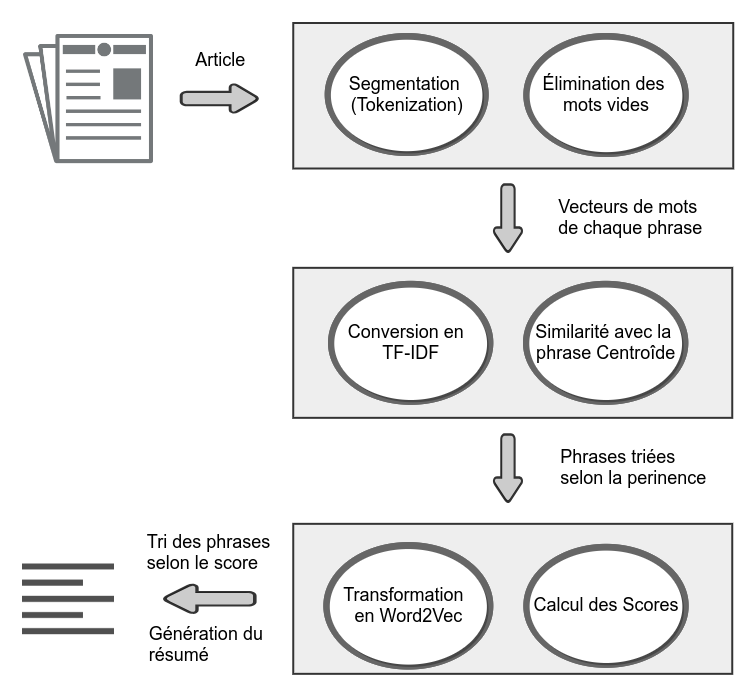
\includegraphics[height=240pt,width=270pt]{img/chapter3/summary.png}
    \caption{Processus de génération de résumé automatique.}
    \label{summaryglobal}
\end{figure}


\subsection{Module de catégorisation}
La catégorisation se fait à l'arrivé d'un nouveau flux d'articles suivant les étapes suivantes (figure \ref{categglobal}) :

\begin{figure}[H]
    \centering
    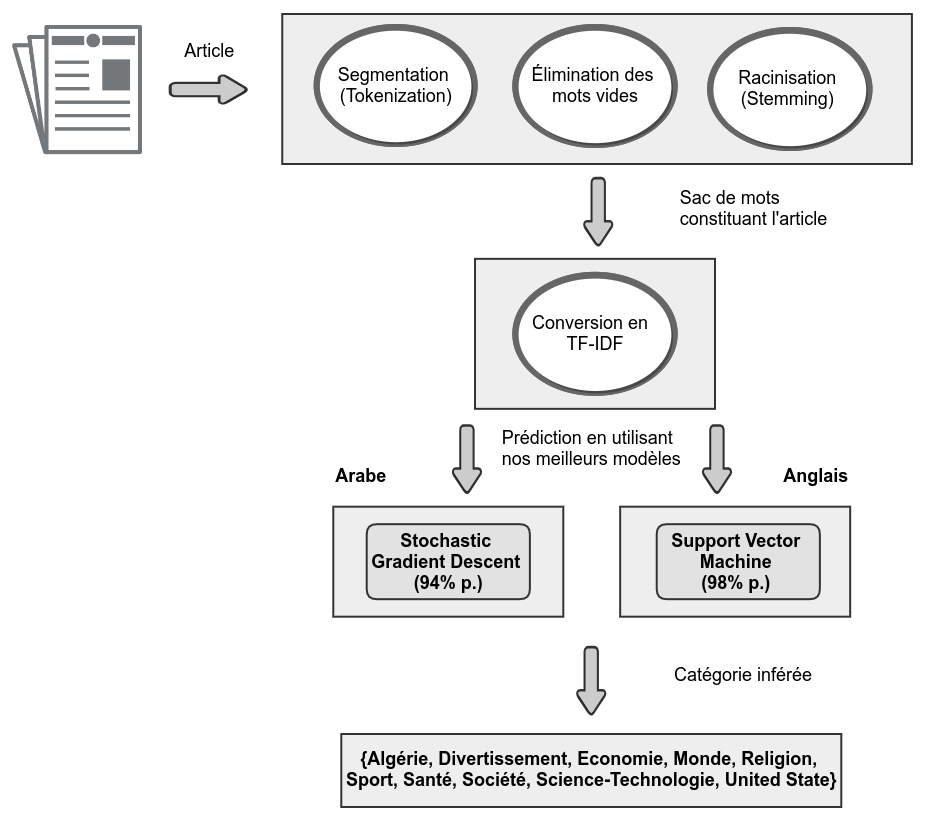
\includegraphics[height=300pt,width=350pt]{img/chapter3/categorization.png}
    \caption{Processus de catégorisation d'articles de presse.}
    \label{categglobal}
\end{figure}

\begin{itemize}
	\item \textbf{Prétraitement des articles:}
	À l'arrivée d'un nouvel article, une phase de pré-traitement est nécessaire, elle comporte les opérations de base du TALN tel que la segmentation, la suppression des mots vide et la racinisation.
    À la fin de cette étape, l'article est prêt à être classifié.\\
    \item \textbf{La classification:}
    Nous avons développé des modèles de classification d'article de presse selon leur contenu. En utilisant les techniques d'apprentissage automatique supervisé, nous avons réussi à obtenir des résultats très satisfaisants (nous allons en discuter dans le chapitre suivant (\emph{Réalisation}\ref{chapter4}).
\end{itemize}

\subsection{Module de traduction automatique}
Dans ce module, notre tâche n'était pas d'implémenter ou de concevoir un traducteur automatique, mais uniquement d'utiliser un traducteur automatique multilingue existant, et de l'intégrer dans notre architecture globale présenté dans la (figure \ref{shemaglobal}). 
Toutefois, il fallait rechercher le module de traduction le plus performant afin de traduire un article complet de la manière la plus rapide.

\section{Architecture fonctionnelle de "Feedny"}

\subsection{Fonctionnement du système}
Deux méthode d'utilisation de notre application sont disponible: Avec authentification, Sans authentification. La personnalisation des recommandations en dépendra.

\subsubsection{Avec authentification (personnalisé)}
Si l'utilisateur s'authentifie, la version personnalisée de notre application lui sera accessible et pourra dès la première connexion choisir ses catégories et ses sources favorites afin de construire son profil utilisateur.

À partir de là, les articles proposés sont choisis en fonction de ses préférences, et les recommandations seront de plus en plus raffinées avec l'utilisation de l'application.

Les utilisateurs de "Feedny" auront comme fonctionnalités:  
\begin{itemize}
	\item \textbf{Catégorisation automatique d'articles:}
	Les articles sont classifiés dans différentes catégories suivant le sujet traité.
	\item \textbf{Résumé automatique:}
	Au lieu de lire un article complet, l'utilisateur aura un résumé généré automatiquement à partir de l'article qui lui permettra de retrouver tout les faits importants décrit dans l'article.
	\item \textbf{Traduction automatique:}
	l'utilisateur aura la possibilité d'avoir une traduction de l'article en cours de lecture.
    \item \textbf{Favoriser un article, une revue ou une catégorie:}
    L'utilisateur pourra aussi marquer un article, une source ou une catégorie précise d'articles comme favorite.
    \item \textbf{Mentionner la satisfaction:}
    Il aura la possibilité d'ajouter une mention de préférence "J'aime" ou "Je n'aime pas" sur la recommandation.
    \item \textbf{Recherche d'articles:}
    l'utilisateur aura la possibilité de faire une recherche spécifique des articles, et ceux en se basant soit sur : une recherche basé mots clés, une recherche basé sur une catégorie ou une recherche selon la source de l'article. 
    \item \textbf{Consultations des articles recommandés:}
    L'interface offrira la possibilité de consulter tout les détails concernant l'article (auteur, date de publication, etc.) 
\end{itemize}
Dès la connexion de l'utilisateur, ce dernier peut s'identifier en utilisant un nom d'utilisateur et un mot de passe ; sinon il utilisera les services non personnalisés du système qui sont présentés dans le point suivant.

\subsubsection{Sans authentification (non personnalisé)}
Dans le cas où l'utilisateur ne souhaite s'identifier, la version non personnalisé sera entièrement accessible et il pourra :
\begin{itemize}
	\item \textbf{Recommandation basée similarité:}
	Dans le cas non personnalisé, la recommandation se basera uniquement sur l'article consulté et lu et les différents articles disponible dans la base de données.	
	\item \textbf{Consultation des articles suggérés:}
	l'utilisateur pourra en effet au moment même ou il lit un article, d'avoir une suggestion d'autres articles jugés similaires par le système.
	\item Toutes les autres fonctionnalités de la version Personnalisé qui n'utilisent pas le profile utilisateur sont également disponible.
\end{itemize}

\section{Vue conceptuel du système "Feedny"}
Nous allons présenté dans cette partie, la façon avec laquelle le logiciel fournit les différentes fonctionnalités. Cette décrit d'une manière claire et précise, le fonctionnement du futur système en utilisant un langage de modélisation. 

Nous avons choisi la méthode UML (Unified Modeling Language), qui est une notation graphique conçue pour représenter, spécifier et construire les systèmes logiciels. UML utilise des techniques orientées objets pour la modélisation des systèmes, depuis la conception jusqu'à la maintenance, d'une manière compréhensible par l'homme et disposant de qualités formelles suffisantes pour être traduites automatiquement en code source.\cite{UML}

\subsection{Diagramme de cas d'utilisation}
"Le diagrammes de cas d'utilisation (initié par Ivar Jacobson en 1992 dans la méthode OOSE) est un type de diagramme UML qui permet de définir les besoins des acteurs dans un système quelconque en établissant les fonctionnalités attendues et en organisant les besoins. Il peut être aussi utilisés ensuite comme moyen d'organisation du développement du logiciel, notamment pour la structuration et le déroulement des tests du logiciel".\cite{UML}

Ces principaux composants sont :

\begin{itemize}
	\item \textbf{Acteur:}
	Un acteur est un utilisateur type qui a toujours le même comportement vis-à-vis d'un cas d'utilisation. Les utilisateurs d'un système appartiennent a une ou plusieurs classes d'acteurs selon les rôles qu'ils tiennent par rapport au système. Il est a noter que, une même personne physique peut se comporter en autant d'acteurs différents que le nombre de rôles qu'elle joue vis-à-vis du système et que un acteur peut aussi être un système externe avec lequel le cas d'utilisation va interagir.\cite{UML}
	\begin{figure}[H]
		\centering
		
\includegraphics[height=55pt,width=40pt]{img/chapter3/acteur.png}
		\caption{Modélisation d'un acteur.}
	\end{figure}
	\item \textbf{Cas d'utilisation:}
	Un cas d'utilisation correspond à un certain nombre d'actions que le système devra exécuter en réponse à un besoin d'un acteur. Un cas d'utilisation doit produire un résultat observable pour les acteurs du système.\cite{UML}
    \begin{figure}[H]
	   \centering
	   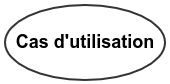
\includegraphics[height=45pt,width=80pt]{img/chapter3/casdutilisation.png}
	   \caption{Modélisation d'un cas d'utilisation.}
    \end{figure}
\end{itemize}

\subsubsection{Diagramme de cas d'utilisation de "Feedny"}
	\begin{figure}[H]
	\centering
	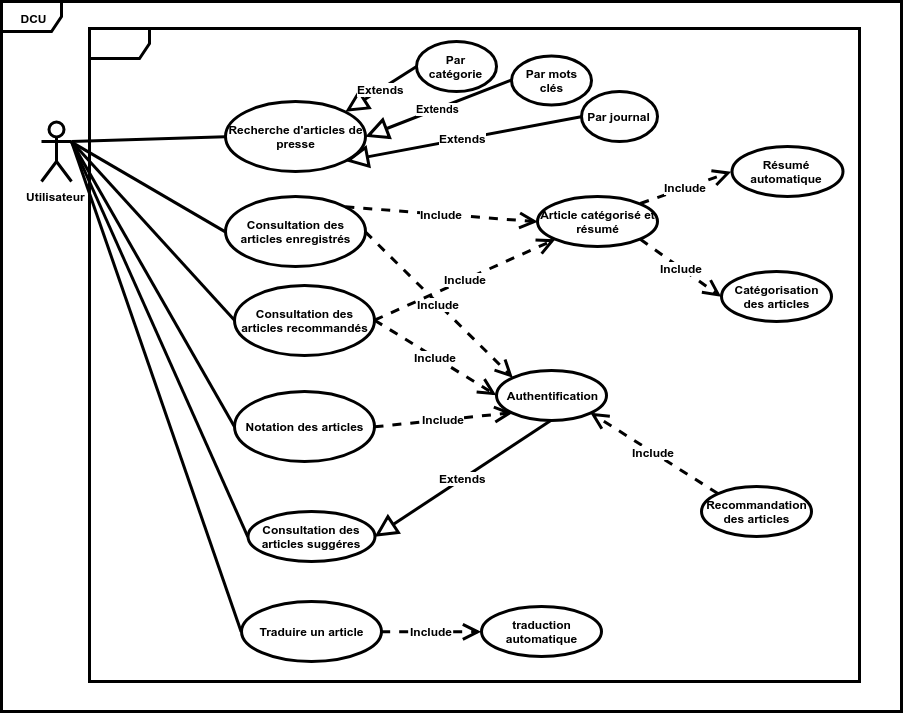
\includegraphics[height=400pt,width=350pt]{img/chapter3/diagcasdutilisation.png}
	\caption{Diagramme présentant les cas d'utilisations}
    \end{figure}

\subsection{Diagramme de classe}
Le diagramme de classe est l'un des pivots essentiels de la modélisation avec UML, il décrit la structure statique du système. En effet, aucun détail ni traitement sont représenté dans ce diagramme puisque il 
se base uniquement sur la notion d'objet, de classe et les différents types d'associations:
\begin{itemize}
	\item \textbf{Classe :} 
    Une classe décrit un groupe d'objets ayant les mêmes propriétés (attributs), un même comportement (opérations), et une sémantique commune (domaine de définition).
	\item \textbf{Objet :} Un objet est l'instance d'une classe, il peut contenir:
        \begin{itemize}
    	\item Attributs : Un attribut est une propriété élémentaire d'une classe. Pour chaque objet d'une classe, l'attribut prend une valeur (sauf cas d'attributs multivalués).
    	\item Méthodes : Une méthode est l'implémentation d'une opération. Chaque classe par défaut inclut plusieurs méthodes, qui décrivent ses opérations.
       \end{itemize}
	\item \textbf{Relations:}
	En UML, il existe plusieurs façons pour décrire les relations entre les classes. Chaque relation exprime un dépendance particulière qui peut être de différents types \cite{UML}:
    	\begin{itemize}
    	\item Association : L'association est le premier niveau de relation entre 2 classes. Elle spécifie tout simplement qu'une classe peut en utiliser une autre. Graphiquement, elle est sous la forme d'un trait plein, jointe à un label décrivant la relation souvent avec un verbe à l'infinitif.
    	\item Agrégation : C'est une relation plus forte qu'une association. Contrairement à l'association,l'agrégation représente une relation d'inclusion structurelle ou comportementale d'un ensemble. De plus, l'agrégation est une relation transitive.
    	\item Composition : Appelée aussi « agrégation composite », elle représente une agrégation particulière. Sa particularité est qu'elle est l'auteur de la création et la destruction d'objets.
    	\item Héritage : C'est un principe abstrait. Il donne la possibilité de diviser récursivement les objets en plusieurs ensembles (parties), où chaque partie est une classe.
       \end{itemize}
\end{itemize}

\subsubsection{Diagramme de classe de "Feedny"}
\begin{figure}[H]
    \centering
    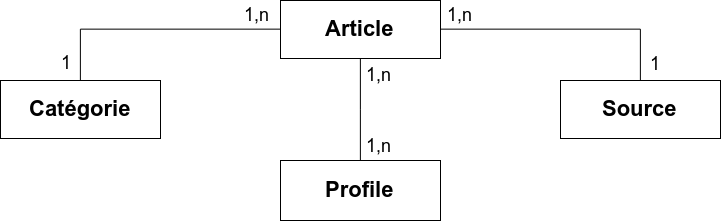
\includegraphics[height=100pt,width=320pt]{img/chapter3/classdiagram.png}
    \caption{Diagramme de classe}
\end{figure}

\subsection{Diagramme de séquence}
Le diagramme de séquence est un diagramme UML qui fait partie des diagrammes comportementaux (dynamiques) dont L'objectif est de représenter les interactions entre les objets et les acteurs ou bien entre objets uniquement  en indiquant la chronologie des échanges. Cette représentation peut se réaliser en considérant les différents scénarios associés.

Un diagramme de séquence est composé d'un ensemble d'objets, où chaque objet a une ligne de vie, ainsi qu'un ensemble de messages. Ces principaux composants sont \cite{UML}:
\begin{itemize}
    \item \textbf{Les Objets :}
    Le diagramme de séquence est composé de plusieurs objets qui interagissent entre eux à l'aide de messages. Un objet est représenté par un rectangle avec le nom de l'objet à l'intérieur.
    \item \textbf{Ligne de vie :}
    Chacun des objets a sa propre ligne de vie, qui peut être considérée comme un axe temporel, elle est représentée par une ligne discontinue. Cette ligne de vie indique la période de vie de l'objet et elle se termine par une croix qui indique la destruction de l'objet.
       \begin{figure}[H]
       	\centering
       	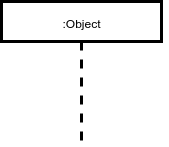
\includegraphics[height=80pt,width=70pt]{img/chapter3/lignevie.png}
       	\caption{Modélisation d'un objet et d'une ligne de vie}
       \end{figure}
    \item \textbf{Les messages :}
     Un message représente une information envoyée de la part d'un objet A à un autre objet B. Il y-a deux types de messages, qui sont les suivants \cite{UML}:
        \begin{itemize}
        \item Messages synchrones : La réception d'un message synchrone provoque un lancement obligatoire d'une de ces méthodes. D'où l'expéditeur reste bloqué jusqu'à la fin de l'exécution de cette méthode et réception d'une réponse. Les messages synchrones sont symbolisés par des flèches en pointillés.
        \item Messages asynchrones : Contrairement aux messages synchrones, l'envoi d'un message asynchrone ne bloque pas l'expéditeur de ce dernier. Ainsi l'expéditeur pourra continuer sa ligne de vie sans avoir à attendre une réponse. Les messages asynchrones sont symbolisés par des flèches pleines.
        \end{itemize}   	
\end{itemize}

\subsubsection{Diagrammes de séquence de "Feedny"}
\begin{figure}[H]
	\centering
	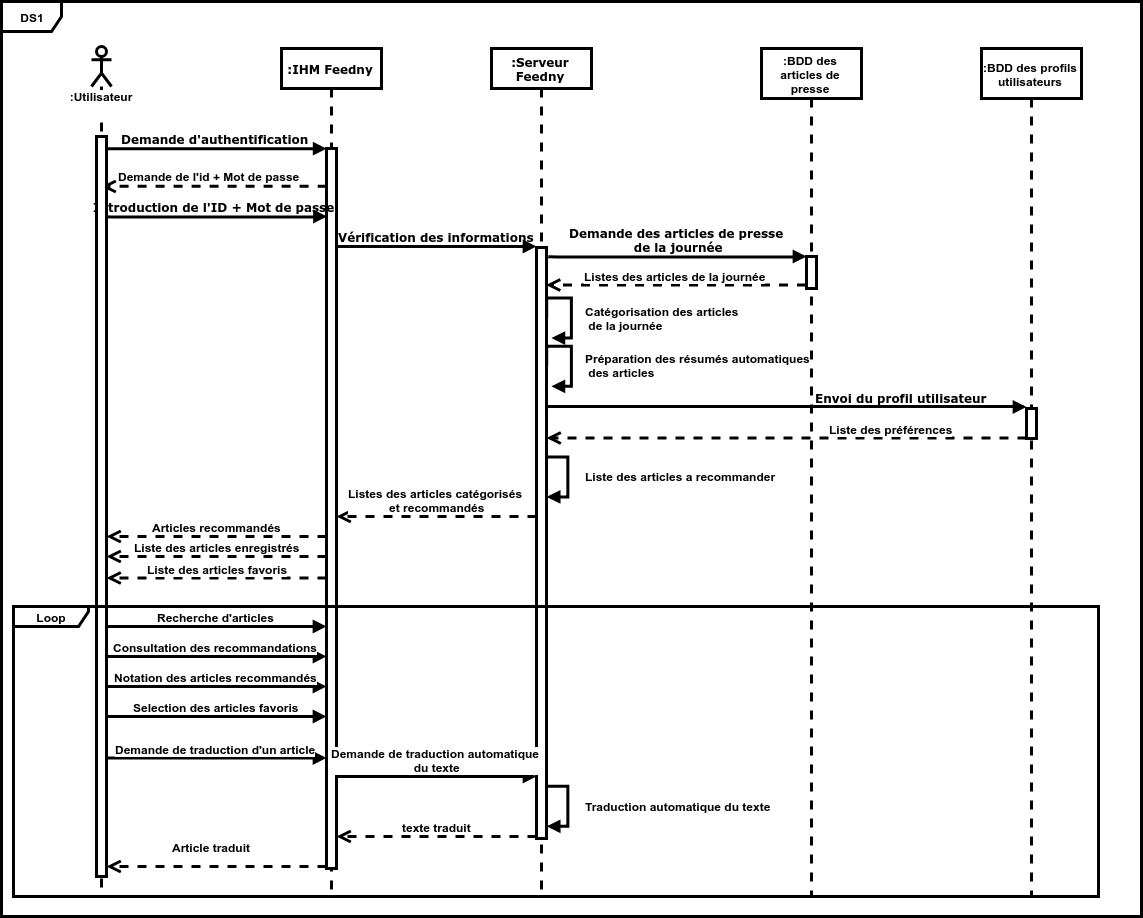
\includegraphics[height=500pt,width=425pt]{img/chapter3/diagseqperso.png}
	\caption{Diagramme de séquence dans le cas personnalisé}
\end{figure}


\begin{figure}[H]
	\centering
	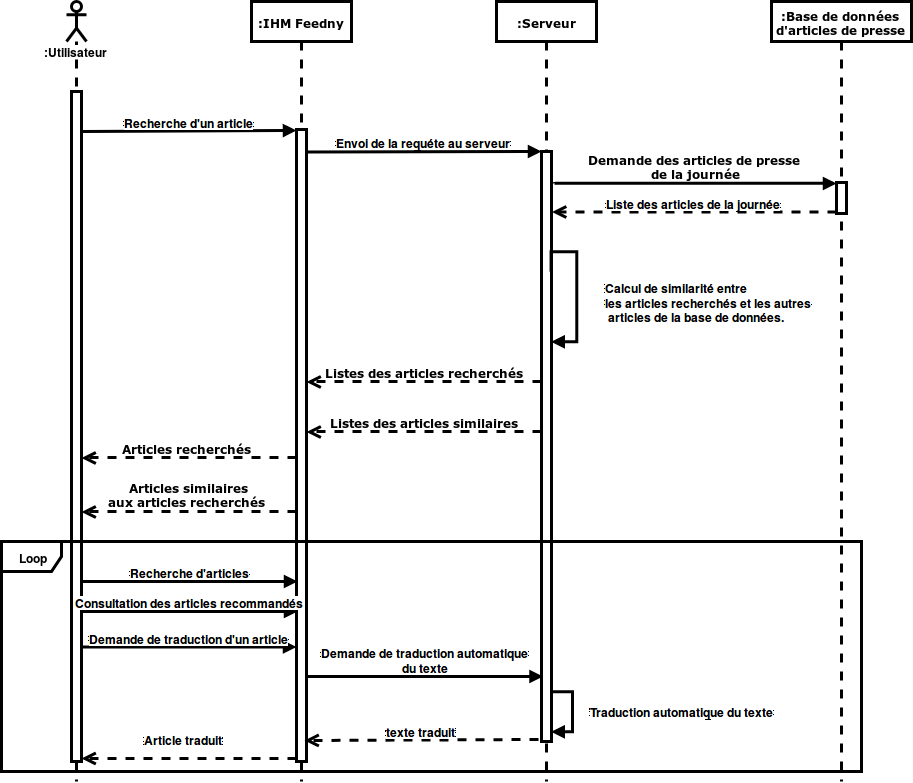
\includegraphics[height=500pt,width=425pt]{img/chapter3/diagseqnonperso.png}
	\caption{Diagramme de séquence dans le cas non personnalisé}
\end{figure}

\section{Conception de la base de données}
\subsection{Bases de données NOSQL}
L'idée de NOSQL a été réintroduite en 2009 lors d'un événement sur la distribution bases de données. À ce moment-là, les principales raisons de passer aux bases de données NOSQL sont reprises: performance et la flexibilité. La performance est principalement axée sur le partage et la gestion des données, tandis que la flexibilité des données correspond aux données semi-structurées ou non structurées qui peut provenir du web. Déjà en 2011 les principales technologies non relationnelles étaient déjà connus et décrits en fonction de leur fonctionnement. Hecht et
Jablonski \cite{NOSQL1} a décrit les principales caractéristiques offertes par différents NOSQL des solutions telles que Voldemort, Redis, Riak, MongoDB, CouchDB, Cassandra, HBase, etc.

À partir de 2012 et jusqu'à aujourd'hui, les bases de données NOSQL ont été de plus en plus évalué et comparé aux SGBDR. Évaluation des performances exécutée par \cite{NOSQL2} comparé Cassandra, MongoDB et PostgreSQL. Il a été conclu que MongoDB est capable de fournir un haut débit, mais surtout quand il est utilisé comme un seul serveur.

MongoDB est une base de données orientée document écrite en C++ \cite{NOSQL3}. Les objets sont stockés en série sous la forme BSON. le
les objets n'ont pas besoin d'avoir la même structure ou les mêmes champs et les champs communs n'ont pas besoin d'avoir le même type,
permettant ainsi un stockage de schéma flexible.A cet effet,nous avons choisi de concevoir une solution basé sur les bases de données NOSQL.

\subsection{Collection Articles}
   \begin{itemize}
     \item \textbf{"\_id" (Identifiant) :} Hash  
     \item \textbf{"language" (Langue) :} ['Ar', 'En']
     \item \textbf{"title" (Titre) :} Chaîne de caractères
     \item \textbf{"source" (Source) :} ['espn', 'bbc-news', 'echourouk', 'elkhabar', etc.]
     \item \textbf{"author" (Auteur) :} Chaîne de caractères
     \item \textbf{"content" (Contenu) :} Texte
     \item \textbf{"publishedAt" (Horaire) :} Timestamp: AAAA-MM-JJTHH:MM:SS
     \item \textbf{Lien de l'"url" (article) :} URL
     \item \textbf{Lien de l'"urlToImage" (image) :} URL 
     \item \textbf{"categoryPredicted" (Catégorie) :} ['sport', 'business', 'religion', etc.]
     \item \textbf{"summaryGenerated" (Résumé) :} Texte
     \item \textbf{"translatedContent" (Traduction) :} Texte
    \end{itemize}

     \begin{lstlisting}[style=code]
      #Exemple d'un document de la collection Articles 
     {
      '_id': '5afc18571d41c833a8632a24', 
      'language': 'en',
      'title': "Smart's stellar Game 2 play draws Cavs praise", 
      'source': 'espn', 
      'author': 'Chris Forsberg', 
      'content': 'LeBron James and Tyronn Lue explain what they think of Marcus...'
      'publishedAt': '2018-05-16T05:48:55Z', 
      'url': 'http://espn.go.com/nba/id/235168',
      'urlToImage': 'http://espn.go.com/nba/id/235168/main.png',  
      'categoryPredicted': 'sport', 
      'summaryGenerated': 'The Celtics improved to 8-2 since Smart returned...', 
      'translatedContent': 'ليبرون جيمس يشرح ما يفكر به من تأثير ماركوس سمارت في نهائيات القسم الشرقي حتى الآن....', 
     },
     \end{lstlisting}

\subsection{Collection Profiles}
\begin{itemize}
     \item \textbf{"\_id" (Identifiant ): } Hash
     \item \textbf{"username" (Nom d'utilisateur) : } Chaîne de caractères
     \item \textbf{"password" (Mot de passe): } Hash
     \item \textbf{"email" (Adreese mail): } Chaîne de caractères
     \item \textbf{"categories" (Catégories): } {catégorie: taux de préférences }
     \item \textbf{"sources" (Sources): } ['bbc-news', 'al-jazeera-english', 'wello-mag', etc.] 
\end{itemize}
\begin{lstlisting}[style=code]
      #Exemple d'un document de la collection Profiles 
     {
      '_id': '5afc18571d41c833a8632a24', 
      'username': 'yankheloufi'
      'password': 'CAESEMgZsfgjSKT7GvZNAtFJaAs'
      'email': 'yk@usthb.dz',
      'categories': {
          'entertainment': '0.63',
          'world': '0.42',
          'health': '0.12',
      },
      'sources': [
            'wello-mag', 'al-jazeera-english', 'bbc-news', 
      ],
     },
     \end{lstlisting}


\section{Formules mathématiques de la recommandation}

\subsection{Recommandation non personnalisé}
La recommandation non personnalisée vise à recommander des articles pour des utilisateurs qui n'ont pas de comptes (non authentifiés), pour cela notre système effectue une recommandation selon le choix de lecture de l'utilisateur, c'est à dire par calcul de similarité entre l'article qui est entrain d'être lu et les articles disponible dans la base de données. Le de calcul de la similarité entre les articles est présenté la dessous:

En considérant P et Q comme des vecteurs, la similarité de cosinus entre une paire de vecteurs lignes p et q est calculée comme suit:

            \[cos(\pmb P, \pmb Q) = \frac {\pmb p \cdot \pmb q}{||\pmb p|| \cdot ||\pmb q||}\]


\subsection{Recommandation personnalisé}
La recommandation des articles aux utilisateurs se base sur les profils de ces derniers. En effet, le profilage utilisateur débute lorsque l'utilisateur s'authentifie pour la première fois et a chaque fois les informations relatives a ses préférences sont récoltés et traités.\\
Cette étape exige:

\subsubsection{Le profilage utilisateur}
Le profilage est la première partie de ce processus. Elle consiste à déterminer les centres d'intérêts d'un utilisateur tout en se basant sur les articles lues par ce dernier. Pour cela, nous avons décidé d'utiliser une méthode de calcul des préférences afin de mieux cibler les utilisateurs et pour garantir une solution conforme aux caractéristiques de la recommandation pour les articles de presse.

\subsubsection{Méthode de calcul des préférences}
Pour le calcul des préférences utilisateurs, nous avons décidé d'utiliser une méthode de calcul qui permet à la fois de résoudre les problèmes de récence et le démarrage à froid. Cette méthode testée s'avère très efficace par rapport aux méthodes existantes et décrites dans le premier chapitre.

Le calcul des valeurs qui représentent les centres d’intérêts et les préférences se fait en utilisant les formules suivantes: 
    Si un article est sélectionné:
                                   \[p = (1-{\alpha}) {p} + {\alpha}\]

    Sinon: 
                                     \[{p} = (1-{\alpha}) {p}\]
Où p est la probabilité de sélection et \alpha  est le degré de diminution du poids.

Dans notre cas:
                                   \[p = 1/{NbC}\]
                                   \[\alpha = 0.1\]

où NbC: Nombre de catégories.\\
Au fur et à mesure, la probabilité de sélection diminue si la catégorie n'est pas sélectionné, et la plus récente aura un poids plus élevé. 
 \begin{algorithm}
	\begin{algorithmic}[1]
		\STATE Profilage
		\STATE Début
		\STATE \alpha \gets 0.1;
		\STATE p \gets 1/$Nombre\_de\_categories$;		
        \STATE dés l'authentification d'un utilisateur i charger ses préférences;
		\STATE préférences \gets préférences(i);	
		\STATE Si $Selection\_article$ Alors:
        \STATE \[p(categorie\_article) \gets (1-{\alpha}) {p} + {\alpha}\]
        \STATE Pour toute catégorie != $categorie\_article$ Faire:
		\STATE \[p(categorie) \gets (1-{\alpha}) {p} \]
        \STATE Fin Pour
		\STATE Fin Si
		\STATE \quad Retourner $Liste\_de\_preferences$	
        \STATE Fin
    \end{algorithmic}
\end{algorithm}
\subsubsection{Méthode de calcul de la similarité entre utilisateurs}
Afin de diversifier la recommandation dans notre système, nous avons mis en place une méthode de calcul de similarité qui permet de recommander des articles par rapport à la similarité entre utilisateurs. Selon \cite{euclidepreuve} qui propose une étude détaillé sur les mesures de similarité pour le filtrage collaboratif, il en est sorti comme conclusion que la distance euclidienne était la mesure la plus adéquate vu sa précision élevée et son temps d'exécution bas par rapport aux autres mesures.\\
En considérant P et Q comme des vecteurs, la distance euclidienne entre une paire de vecteurs lignes p et q est calculée comme suit:
            \[d({p} ,{q})=d({q} ,{p})={\sqrt {(q_{1}-p_{1})^{2}+(q_{2}-p_{2})^{2}+\cdots +(q_{n}-p_{n})^{2}}}\\
            ={\sqrt {\sum _{i=1}^{n}(q_{i}-p_{i})^{2}}}\]
\begin{algorithm}[H]
	\begin{algorithmic}[1]
        \STATE Diversité
        \STATE Début
		\STATE dés l'authentification d'un utilisateur i charger ses préférences;
		\STATE préférences = préférences(i);
		\STATE Pour chaque article dans la base des articles Faire:
        \STATE Si {$Distance\_euclidienne(i,j) >= Seuil(j)$} Alors:
        \STATE Ajouter les 2 centres d'intérêts de l'utilisateur \textbf{j} au préférences de l'utilisateur \textbf{i};
 		\STATE Fin Si;	
		\STATE Fin Pour;
		\STATE \quad Retourner $Liste\_de\_preferences\_diversifier$
		\STATE Fin
	\end{algorithmic}
\end{algorithm}

\subsubsection{Processus de recommandation}
\begin{algorithm}[H]
	\begin{algorithmic}[1]
		\STATE Recommandation
		\STATE Début
		\STATE dés l'authentification d'un utilisateur \textbf{i} charger ses préférences ;\\
		\STATE Profilage(i) ;\\
		\STATE Diversité(i) ;\\
		\STATE Pour chaque article dans la base des articles Faire:
		$Liste_recommandations \gets article$;\\
		\STATE FinSI;
		\STATE FinPour;
		\STATE \quad Retourner $Liste\_de\_recommandations$;
		\STATE Fin
	\end{algorithmic}
\end{algorithm}

\section{Conception de la Catégorisation d'articles}
En se bansant sur les travaux de \cite{categorisation} pour l'Anglais et \cite{categorisation} pour l'Arabe, nous avons entrainé nos modèles sur des corpus d'articles de différentes sources afin de garantir la diversité dans nos données (plus de détails dans le chapitre 4\ref{chapter4}).
À REVOIR!!
\subsubsection{Processus de catégorisation}
    \begin{algorithm}[H]
        \begin{algorithmic}[1]
        \STATE Algorithme
        \STATE Début
        \STATE Chargement du l'article;\\
        \STATE Prétraitement: Tokenisation, élimination des mots vides, racinisation ;\\
        \STATE Calcul de la fréquence des termes par document TF-IDF ;\\
        \STATE Prédiction de la catégorie;\\
        \STATE \quad Retourner Modèle;
        \STATE Fin
        \end{algorithmic}
    \end{algorithm}


\section{Conception du module de résumé automatique}
Pour ce module de résumé automatique, nous avons choisi un résumeur automatique extractif de \cite{notrerésumé} qui est basé sur les plongements de mots (Word embeddings) décrit dans le chapitre précédent.

\subsection{Prétraitement des articles}
Dans cette phase , il suffit juste de tokeniser le texte et supprimer les mots vides puisque le stemming ne peut pas être utilisé. Pour cause, le plongement de mots qu'on va utiliser (le modèle skip-gram entrainé sur le contenu Wikipédia) servira entre autre a détecté les régularités linguistiques des des mots de la même racine.

\begin{algorithm}[H]
	\begin{algorithmic}[1]

\STATE Prétraitement
\STATE Début
\STATE Chargement du document;
\STATE Extraction des phrases ;
\STATE Tokenisation ;
\STATE Suppression des mots vides;
\STATE \quad Retourner $Document_traité$;
\STATE Fin

\end{algorithmic}
\end{algorithm}

\subsection{Construction d'un vecteur de centroïde}
Afin de construire un vecteur centroïde en utilisant les plongement de mots, nous sélectionnons d'abord les mots significatifs dans le document. Pour cela, nous sélectionnons mots ayant le poids Tf-IDF supérieur à un seuil de document (idf). Ainsi, nous calculons l'encastrement du centroïde comme la somme des mots les mieux classés dans le document en utilisant les plongements de mots de Wikipédia (environ 1 million de mots). 

\begin{algorithm}[H]
	\begin{algorithmic}[1]
		\STATE Recommandation
		\STATE Début
		\STATE Lecture du seuil idf fixé;
		\STATE Calcul du tf-idf de chaque terme dans le document ;
		\STATE Pour chaque terme dans le document Faire:
		\STATE SI tf-idf(terme) >= seuil Alors:
		\STATE    $Liste_des_mots_importants$ \gets terme;
		\STATE FinsI;
		\STATE FinPour;
		\STATE \quad Retourner $Liste_des_mots_importants$;
		\STATE Fin
	\end{algorithmic}
\end{algorithm}


\subsection{Notation des phrases}
Dans ce processus, pour chaque phrase du document on additionne les plongement de mots de chaque terme de telle façon a avoir un une représentation sur laquelle la phrase est représenté par un score. Ainsi, la phrase ayant le score le plus élevé désigne la phrase centroid.\\
Il est a noter que les vecteurs a additionné sont calculé sur la base du modèle Word2Vec pré entrainé sur le contenu de Wikipédia.

\begin{algorithm}[H]
	\begin{algorithmic}[1]
		\STATE Notation
		\STATE Début
		\STATE Lecture du vecteur de centroïde;
		\STATE Calcul de score pour chaque phrase;
		\STATE \quad Retourner $Notations$;
		\STATE Fin
	\end{algorithmic}
\end{algorithm}


\subsection{Séléction des phrases}
Pour chaque phrase du document, on calcule la \emph{similarité de cosinus} entre elle et la phrase centroïde du document. Les phrases sont ensuite triées par ordre décroissant de leurs scores de similarité. Les phrases les mieux classées sont itérativement sélectionnés et ajoutés au résumé jusqu'à ce que la limite (taille du résumé) soit atteinte. Afin de satisfaire la propriété de redondance, au cours de chaque itération nous allons calculer la \emph{similarité de cosinus} entre la phrase a venir et chacune déjà dans le résumé.
Il est a noter qu' un seuil a été fixé afin de rejeter toutes les phrases qui ont une similarité très élevé par rapport a une phrase afin d'éviter cette redondance.

\begin{algorithm}[H]
	\begin{algorithmic}[1]
		\STATE Séléction
		\STATE Début
		\STATE Lecture du seuil de résumé fixé;
		\STATE Lecture du seuil de similarité fixé;
		\STATE Tant que le seuil du résumé est non atteint Faire :
		\STATE similarité entre la phrase actuelle et la phrase centroïde \gets \[cos(\pmb P, \pmb C\];
		\STATE similarité de cosinus entre la phrase actuelle et celle du résumé  \gets \[cos(\pmb P, \pmb R\]	
		\STATE Si (\[cos(\pmb P, \pmb R\] <= seuil de similarité et \[cos(\pmb P, \pmb C\] <= seuil de similarité) Alors :
		\STATE $phrases_résumé \gets phrase_actuelle$
		\STATE Finsi
		\STATE Fintantque;	
		\STATE \quad Retourner $phrases_résumés$;
		\STATE Fin
	\end{algorithmic}
\end{algorithm}

\subsection{Algorithme du résumeur automatique extractif}

\begin{algorithm}[H]
	\begin{algorithmic}[1]
\STATE résumé
\STATE Début
\STATE Chargement du document ;
\STATE Lecture des paramètres ;
\STATE Prétraitement de l'article ;
\STATE Construction du vecteur de centroide selon le modèle de plongement de mots pré entrainé de Wikipédia;
\STATE Notation des phrases;
\STATE Séléction des phrases pertinentes;
\STATE Ordonnancement des phrases selon leur rang dans le document;
\STATE \quad Retourner résumé;
\STATE Fin 
   \end{algorithmic}
\end{algorithm}


\section{Conclusion}
Lors de ce chapitre, nous avons proposé l'architecture du système "Feedny" et décrit ses modules, par la suite nous avons proposé une conception détaillé de notre application. Dans le chapitre qui suit, nous allons réaliser la conception de cette architecture.